\documentclass[../main.tex]{subfiles}
\graphicspath{{\subfix{../pictures/}}}
\begin{document}

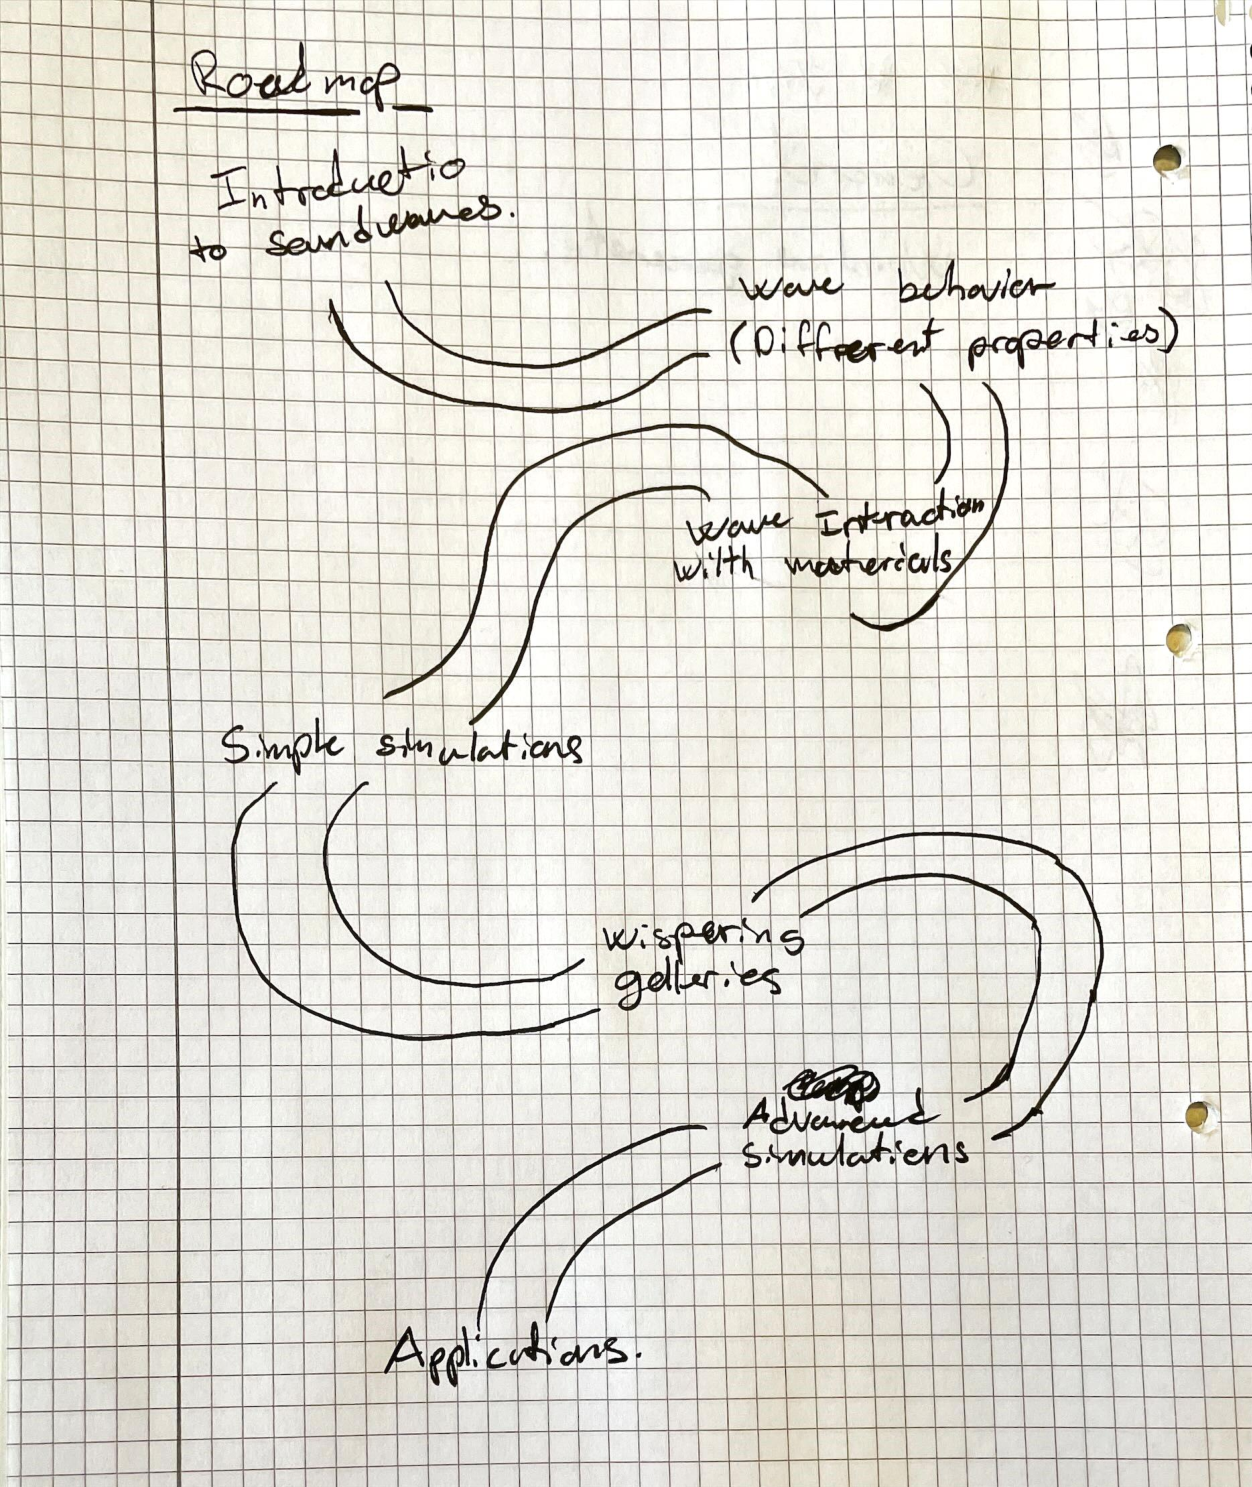
\includepdf[height=1.5\textwidth]{pictures/Roadmap.pdf}

\section{Roadmap}

\subsection{What to do}

\begin{itemize}
    \item \#: 2-days in the week
    \item ¤: Whole week free
\end{itemize}

\begin{itemize}
    \item [\textbf{Week 6: \#}] Write disposition and roadmap (This)
    \item [\textbf{Week 7: \#}] Read up on Sound in General 
    \item [\textbf{Week 8: \#}] Read up on Sound behavior and properties (Somewhat the same as (1)) 
    \item [\textbf{Week 9-10: \#}] Write down something and begin the simulation part and still reading
    \item [\textbf{Week 11: \#}] Read what you feel you are missing (And writting) 
    \item [\textbf{Week 12-16: \#}] Whispering gallery part Read a lot and try to deduct the formulas
    \item [\textbf{Week 17-18: \#}] Simulation
    \item [\textbf{Week 19: \#}] Exams
    \item [\textbf{Week 20: \#}] Exams
    \item [\textbf{Week 21: \#}] Exams - And get back up. Get into it again (Simulation)
    \item [\textbf{Week 22: ¤}] Buffer
    \item [\textbf{Week 23: ¤}] Application
    \item [\textbf{Week 24: ¤}] All the boring stuff
    \item [\textbf{Week 25: ¤}] Hand in $\checkmark$
\end{itemize}

\subsection{Direction of Article}
\begin{itemize}
    \item Introduction to Soundwaves
    \begin{itemize}
        \item Short and compact introduction
        \item Wave equation
    \end{itemize}
    \item Wave Behavior
    \begin{itemize}
        \item Extension of the point before. But going in-depth with the attributes of different wave properties
    \end{itemize}
    \item Wave interaction with materials
    \begin{itemize}
        \item Description of different behaviors of different attributes
        \item Boundary Constraints
    \end{itemize}
    \item Simple simulation
    \begin{itemize}
        \item Simulating wave on $\mathbb{R}^n_+$ with different boundary conditions and wave properties as found in previous
    \end{itemize}
    \item Echo
    \begin{itemize}
        \item Description of echo just in short term
    \end{itemize}
    \item Whispering Galleries $(*)$
    \begin{itemize}
        \item description of the gallery effect and what wave and boundary conditions we need to get this effect.
        \item examples of of this
    \end{itemize}
    \item  Advance simulation
    \begin{itemize}
        \item Simulation of the effect, with different types of shapes, including conditions where we do not expect this to happen.
    \end{itemize}
    \item Application
    \begin{itemize}
        \item What I found, refind the medical application with electrowaves.
    \end{itemize}
\end{itemize}


\end{document}